\documentclass{sig-alternate}
\usepackage[utf8]{inputenc}

\usepackage{amsmath,amssymb}
\usepackage{amsrefs}
\usepackage[usenames,dvipsnames]{color}
\usepackage{stmaryrd}
\usepackage{enumerate}
\usepackage[algoruled,vlined,english,linesnumbered]{algorithm2e}
\usepackage[pdfpagelabels,colorlinks=true,citecolor=blue]{hyperref}
\usepackage{comment}
\usepackage{multirow}
\usepackage{tikz}

\newcommand{\noopsort}[1]{}
\DeclareMathOperator{\NP}{NP}
\DeclareMathOperator{\HP}{HP}
\DeclareMathOperator{\PP}{PP}
\DeclareMathOperator{\Hom}{Hom}
\DeclareMathOperator{\End}{End}
\DeclareMathOperator{\GL}{GL}
\DeclareMathOperator{\val}{val}
\DeclareMathOperator{\pr}{pr}
\DeclareMathOperator{\tr}{Tr}
\DeclareMathOperator{\com}{Com}
\DeclareMathOperator{\Grass}{Grass}
\DeclareMathOperator{\Lat}{Lat}
\DeclareMathOperator{\round}{round}


\newtheorem{theo}{Theorem}[section]
\newtheorem{lem}[theo]{Lemma}
\newtheorem{prop}[theo]{Proposition}
\newtheorem{cor}[theo]{Corollary}
\newtheorem{quest}[theo]{Question}
\newtheorem{conj}[theo]{Conjecture}
%\theoremstyle{definition}
\newtheorem{rem}[theo]{Remark}
\newtheorem{ex}[theo]{Example}
\newtheorem{deftn}[theo]{Definition}
\newtheorem{rmk}[theo]{Remark}

\newcommand{\N}{\mathbb N}
\newcommand{\Z}{\mathbb Z}
\newcommand{\Zp}{\Z_p}
\newcommand{\Q}{\mathbb Q}
\newcommand{\Qp}{\Q_p}
\newcommand{\Fp}{\mathbb{F}_p}
\newcommand{\R}{\mathbb R}
\renewcommand{\O}{\mathcal O}
\newcommand{\OK}{\mathcal{O}_K}
\newcommand{\XX}{\mathbf X}
\newcommand{\trans}{{}^{\text t}}
\newcommand{\T}{\mathcal{T}}

\renewcommand{\prec}{\text{\rm prec}}

\newcommand{\id}{\textrm{id}}
\newcommand{\Epi}{\textrm{Epi}}
\renewcommand{\c}{\text{\rm c}}

\newcommand{\detp}{\det{'}}
\newcommand{\low}{\text{\rm low}}
\newcommand{\up}{\text{\rm up}}
\newcommand{\DI}{\text{\rm DI}}
\newcommand{\II}{\text{\rm II}}
\DeclareMathOperator{\charpoly}{char}
\newcommand{\charp}{\charpoly'}

\newcommand{\lb}{\ensuremath{\llbracket}}
\newcommand{\rb}{\ensuremath{\rrbracket}}
\newcommand{\lp}{(\!(}
\newcommand{\rp}{)\!)}
\newcommand{\col}{\: : \:}

\def\todo#1{\ \!\!{\color{red} #1}}
\definecolor{purple}{rgb}{0.6,0,0.6}
\def\todofor#1#2{\ \!\!{\color{purple} {\bf #1}: #2}}

\def\binom#1#2{\Big(\begin{array}{cc} #1 \\ #2 \end{array}\Big)}

\begin{document}


\title{p-adic stability in linear algebra}

\numberofauthors{3}
\author{
\alignauthor Xavier Caruso\\
  \affaddr{Universit\'e Rennes 1}\\
  \email{\normalsize \textsf{xavier.caruso@normalesup.org}}
\alignauthor Tristan Vaccon\\
  \affaddr{Universit\'e Rennes 1}\\
  \email{\normalsize \textsf{tristan.vaccon@univ-rennes1.fr}}
\alignauthor David Roe \\
  \affaddr{University of British Columbia}\\
  \email{\normalsize \textsf{roed.math@gmail.com}}
}

\maketitle

\begin{abstract}
Using the differential precision methods developed previously by the same authors,
we study the $p$-adic stability of standard operations on matrices and vector 
spaces. We demonstrate that lattice-based methods surpass naive methods in many
applications, such as matrix multiplication and sums and intersections of subspaces.
We also analyze determinants, characteristic polynomials and LU factorization using these differential methods.
We supplement our observations with numerical experiments.
\end{abstract}

\vspace{1mm}
 \noindent
 {\bf Categories and Subject Descriptors:} \\
\noindent I.1.2 [{\bf Computing Methodologies}]:{~} Symbolic and Algebraic
  Manipulation -- \emph{Algebraic Algorithms}

 \vspace{1mm}
 \noindent
 {\bf General Terms:} Algorithms, Theory

 \vspace{1mm}
 \noindent
 {\bf Keywords:} $p$-adic precision
\medskip

\section{Introduction}

For about twenty years, the use of $p$-adic methods in symbolic 
computation has been gaining popularity: they were successfully 
used for instance 
to compute compose products of polynomials 
\cite{boston-gonzalez-perdry-schost:05a}, 
to produce hyperelliptic curves of genus $2$ with complex multiplication 
\cite{gaudry-houtmann-weng-ritzenthaler-kohel:06a},
to compute isogenies between elliptic curves \cite{lercier-sirvent:08a} 
and, last but not least,
to count points on certain varieties (mainly curves) using $p$-adic 
cohomology theories (\emph{cf} \cite{kedlaya:01a,lauder:04a} and many
followers).
However, a general framework allowing a precise study of $p$-adic 
precision --- which is a main issue we encounter when trying to work 
with $p$-adic numbers --- was designed only recently in 
\cite{caruso-roe-vaccon:14a}. 

\todo{Rewrite the introduction}

\begin{comment}
The present paper, which may be considered as a continuation of 
\cite{caruso-roe-vaccon:14a}, aims at using the theory of \emph{loc. 
cit.} in order to analyze the $p$-adic stability of many standard 
algorithms for computing with basic algebraic structures: numbers, 
matrices, univariate polynomials and vector spaces. For each considered 
algorithm, we will follow the same protocol: 
first, we will compute the theoretical loss of precision of the 
underlying question using the framework of \cite{caruso-roe-vaccon:14a} 
and then compare it to those observed in available implementations in 
\textsc{pari} \cite{pari}, \textsc{magma} \cite{magma} and/or 
\textsc{sage} \cite{sage}.

The conclusion of our analysis is that generic algorithms which are 
designed to work over an arbitrary field are often quite unstable. Very 
roughly, denoting by $D$ the number of divisions performed by the 
algorithm under analysis and by $q$ the cardinality of the residue 
field, it appears that the numbers of lost digits is about $O(\frac D 
q)$ whereas the theoretical loss of precision is closer than $O(\log_q 
D)$ --- and sometimes even $O(1)$. We would like to underline in 
particular that the instability phenomema are much more apparent when 
the residue field is small. It is the reason why we will always take
$K = \Q_2$ is our examples.
\end{comment}

\medskip

\noindent
{\bf Organization of the paper.}
The section \ref{sec:theory} introduces the theory of ultrametric 
precision developed in \cite{caruso-roe-vaccon:14a} and completes 
it on a technical point.
In \S \ref{sec:matrices}, we focus on matrices... \todo{Complete
this}.

\medskip

\noindent
{\bf Notations.}
Throughout the paper, the letter $K$ will refer to a complete 
discrete valuation field of characteristic $0$, that is either a finite 
extension of the field of $p$-adic numbers $\Qp$ or a field of Laurent 
series over a field of characteristic $0$ \todo{what about mixed characteristic with infinite residue field?}.
We denote by $\val : K \to \Z 
\cup \{+\infty\}$ of $K$ --- it is the $p$-adic valuation when $K = \Qp$ 
and the usual valuation of a Laurent series when $K = k((t))$ --- and by 
$\Vert \cdot \Vert$ the corresponding norm.

\section{The theory of p-adic precision}
\label{sec:theory}

The aim of this section is to summarize briefly the content of 
\cite{caruso-roe-vaccon:14a} and complete it on certain points.

\subsection{Lattices as precision data}

Roughly speaking, the main proposal of \cite{caruso-roe-vaccon:14a} is 
to use lattices to track precision when computing with elements lying in 
vector spaces over $K$.

To make this sentence more explicit, let us consider a finite 
dimensional\footnote{The framework of \cite{caruso-roe-vaccon:14a} is 
actually those of Banach spaces. However we will not need infinite 
dimensional spaces in the present paper.} normed vector space $E$ 
defined over $K$. We use the notation $\Vert \cdot \Vert_E$ for the norm 
on $E$ and $B^-_E(r)$ (resp. $B^{\phantom -}_E(r)$) for the open (resp. 
closed) ball of radius $r$ centered at the origin. A lattice $L \subset 
E$ is, by definition, a sub-$\O_K$-module which generates $E$ over $K$. 
Since we are working in a ultrametric world, the balls $B^{\phantom 
-}_E(r)$ and $B^-_E(r)$ are examples of lattices. Actually, lattices 
should be thought as special neighborhoods of $0$ and therefore are good 
candidates to model precision data. Moreover, as revealed in 
\cite{caruso-roe-vaccon:14a}, they behave quite well under (strictly) 
differentiable maps:

\begin{prop}
\label{prop:precision}
Let $E$ and $F$ be two finite dimensional normed vector spaces over $K$ 
and $f : U \rightarrow F$ be a function defined on an open subset $U$ of 
$E$. We assume that $f$ is differentiable at some point $v_0 \in U$ and 
that the differential $f'(v_0)$ is surjective.
Then, for all $\rho \in (0, 1]$, there exists a positive real
number $\delta$ such that, for all $r \in (0, \delta)$, any lattice
$H$ such that $B^-_E(\rho r) \subset H \subset B^{\phantom -}_E(r)$ 
satisfies:
\begin{equation}
\label{eq:firstorder}
f(v_0 + H) = f(v_0) + f'(v_0) (H).
\end{equation}
\end{prop}

Proposition \ref{prop:precision} can be rephrased in terms of precision 
as follows: if the input $v_0$ is known at precision $H$, then $f(v_0)$ 
is known up to $f'(v_0)(H)$ and this precision is optimal. Optimality is 
reflected by the equality sign in Eq.~\eqref{eq:firstorder}.

In \cite{caruso-roe-vaccon:14a}, we also explained that if the function 
$f$ is locally analytic, then the constant $\delta$ appearing in
Proposition \ref{prop:precision} can be made explicit in terms of the
growing function $\Lambda(f)$ of $f$ defined by:
$$\textstyle \Lambda(f)(v) = 
\log \big( \sup_{h \in B^-_E(e^v)} \Vert 
f(h) \Vert \big)$$
with the convention that $\Lambda(f)(v) = +\infty$ if $f$ does not
converge on $B^-_E(e^v)$.
We refer to \cite[Proposition 3.12]{caruso-roe-vaccon:14a} for the
precise statement and seek here to state the particular case of
integral polynomial functions. A function $f : E \to F$ is said 
\emph{integral polynomial} if it is given by multivariate polynomial 
functions with coefficients in $\O_K$ in any (equivalently all) system 
of coordinates associated to orthonormal bases.

\begin{prop}
\label{prop:precision2}
We keep the notations of Proposition \ref{prop:precision} and assume 
in addition that $f$ is integral polynomial. Let $C$ be a positive real
number such that $B_F(1) \subset f'(v_0)(B_E(C))$. 
Then Proposition \ref{prop:precision} holds with $\delta = C \cdot
\rho^{-1}$.
\end{prop}

In \cite[Appendix A]{caruso-roe-vaccon:14a}, the theory is extended 
to manifolds over $K$ and covers this way a very large families of
situations (\emph{e.g.} computation with vector spaces as discussed
in \S \ref{sec:vectorspaces}). In this extended framework, the precision 
datum at some point $x$ is a lattice in the tangent space at $x$. 
Propositions \ref{prop:precision} and \ref{prop:precision2} have
analogues as well, simply obtained by working in charts.

\subsection{A bound on a growing function}
\label{ssec:boundLambdaf}

In the next sections, we will compute the derivative of several standard 
operations and remark that it sometimes has a simple expression in term 
of the input and the output. In other terms, the function $f$ modeling
such an operation satisfies a differential equation of the form
$f' = g \circ (f, \id)$
where $g$ is a given --- and hopefully rather simple --- function. The 
aim of this subsection is to study this differential equation and to 
derive from it some bounds on the growing function $\Lambda(f)$. 
\emph{In the following, we shall always assume that $K$ has 
characteristic $0$.}

We actually generalize a bit the setting above and consider the 
differential equation:
\begin{equation}
\label{eq:diffequah}
f' = g \circ (f, h).
\end{equation}
Here $g$ and $h$ are known locally analytic functions and $f$ is the 
unknown, which is assumed to be locally analytic as well. The function
$f$ goes from $U$ to $V$, two open subsets in two finite dimensional
normed vector spaces $E$ 
and $F$ respectively. The function $h$ goes from $U$ to $W$ where $W$
is again an open subset in a normed $K$-vector space $G$. Consequently,
$g$ goes from $V \times W$ to the vector space $\Hom(E,F)$ of
(continuous) linear maps $E \to F$.
In what follows, we always assume that $V$ and $W$ contain the origin, 
$f(0) = 0$, $h(0) = 0$ and $g(0) \neq 0$. There assumptions are harmless 
for two reasons: first, we can always shift $f$ and $h$ (and $g$ 
accordingly) so that they both vanish at $0$ and second, in order to 
apply Proposition \ref{prop:precision2}, the derivative $f'(0)$ 
needs to be surjective and therefore \emph{a fortiori} nonzero.

We assume that we are given in addition two nondecreasing convex 
functions $\Lambda_g$ and $\Lambda_h$ such that $\Lambda(g) \leq 
\Lambda_g$ and $\Lambda(h) \leq \Lambda_h$. We suppose further that 
there exists $\nu$ such that $\Lambda_g$ is constant on the interval 
$({-}\infty, \nu]$\footnote{We note that this assumption is fullfilled if 
we take $\Lambda_g = \Lambda(g)$ because we have assumed that $g(0)$ 
does not vanish.}. We introduce the functions $\tau_\nu$ and $\Lambda_f$ 
defined by:
$$\begin{array}{rll}
&\tau_\nu(x) = x & \text{if } x \leq \nu \\
& \hphantom{\tau_\nu(x)} = {+} \infty & \text{otherwise} \medskip \\
\text{and} &
\multicolumn{2}{l}{\Lambda_f(x) = 
  \tau_\nu \circ (\id + \Lambda_g \circ \Lambda_h)(x + \alpha)}
\end{array}$$
where $\alpha$ is a real number satisfying $\Vert n! \Vert \geq 
e^{-\alpha n}$ for all $n$. If $p$ is the characteristic of the residue field,
a suitable value for $\alpha$ is $\alpha = - 
\frac p {p-1} \cdot \log \Vert p \Vert$ if $p > 0$ and $\alpha = 0$ if $p = 0$.
The next Proposition is proved in Appendix \ref{app:proof}.

\begin{prop}
\label{prop:boundLambdaf} \label{PROP:BOUNDLAMBDAF}
We have $\Lambda(f) \leq \Lambda_f$.
\end{prop}

\begin{figure}
\null \hfill
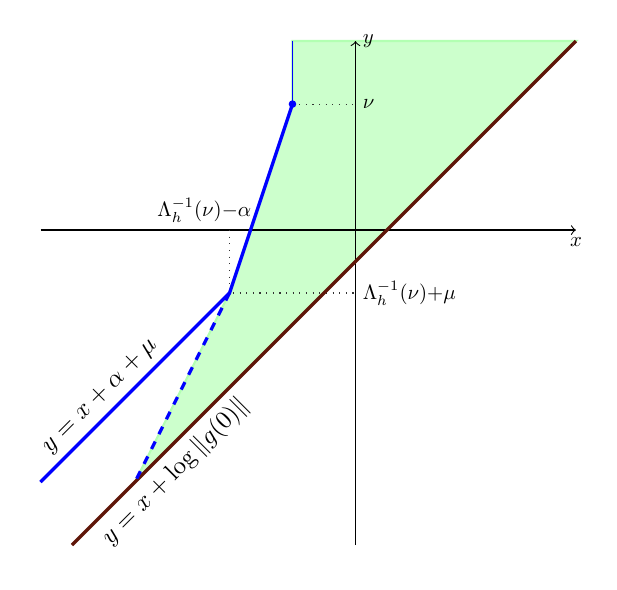
\begin{tikzpicture}[scale=0.8]
\draw[thick,green!30,fill=green!20] 
   (-2,-1)--(-1,2)--(-1,3)--(3.5,3)
 --(2.5,2)--(-3.5,-4)--cycle;
\draw[->] (-5,0)--(3.5,0);
\draw[->] (0,-5)--(0,3);
\node[below, scale=0.75] at (3.5,0) { $x$ };
\node[right, scale=0.75] at (0,3) { $y$ };
\draw[black!80,dotted] (-1,2)--(0,2);
\node[right,scale=0.75] at (0,2) { $\nu$ };
\draw[black!80,dotted] (-2,0)--(-2,-1)--(0,-1);
\node[above,scale=0.75] at (-2.4,0) { $\Lambda_h^{-1}(\nu){-}\alpha$ };
\node[right,scale=0.75] at (0,-1) { $\Lambda_h^{-1}(\nu){+}\mu$ };
\draw[Blue,very thick] (-5,-4)--(-2,-1)--(-1,2);
\fill[Blue] (-1,2) circle (0.06);
\draw[Blue] (-1,2)--(-1,3);
\draw[Sepia, very thick] (-4.5,-5)--(3.5,3);
\draw[Blue, very thick,dashed] (-2,-1)--(-3.5,-4);
\node[below right,rotate=45,scale=0.9] at (-4.3,-4.8) 
  { $y = x + \log \Vert g(0) \Vert$ };
\node[above right,rotate=45,scale=0.9] at (-4.8,-3.8) 
  { $y = x + \alpha + \mu$ };
\end{tikzpicture}
\hfill \null

\caption{Admissible region for the graph of $\Lambda(f)$}
\label{fig:area}
\end{figure}

Figure \ref{fig:area} illustrates Proposition \ref{prop:boundLambdaf}. 
The blue plain line represents the graph of the function $\Lambda_f$. A 
quick computation shows that, on a neighborhood of ${-}\infty$, this 
function is given by $\Lambda_f(x) = x + \alpha + \mu$
where $\mu$ is the value that $\Lambda_g$ takes on the interval 
$({-}\infty, \nu]$. Proposition \ref{prop:boundLambdaf} says that the
graph of $\Lambda(f)$ lies below the plain blue line. We remark
moreover that the Taylor expansion of $f(z)$ starts with the term
$g(0) z$. Hence, on a neighborhood on ${-}\infty$, we have 
$\Lambda(f)(x) = x + \log \Vert g(0) \Vert$. Using convexity, we 
get:
$$\Lambda(f)(x) \geq x + \log \Vert g(0) \Vert, 
  \quad \forall x \in \R.$$
In other words, the graph of $\Lambda(f)$ lies above the brown line.
Furthermore, we know that the slopes of $\Lambda(f)$ are all integral
because $f$ is locally analytic. Hence, $\Lambda(f)$ cannot lie above
the dashed blue line defined as the line of slope $2$ passing through
the first break point of the blue plain line --- which has coordinate 
$(y_0 - \alpha - \mu, y_0)$ with $y_0 = \min(\Lambda_h^{-1}(\nu) + \mu, 
\nu)$. As a conclusion, we have proved that the graph of $\Lambda(f)$ 
must coincide with the brown line until it meets the dashed blue line 
and then has to stay in the green area.

As a consequence of the above discussion, we derive the following 
proposition which can be directly combined with Proposition 3.12 of 
\cite{caruso-roe-vaccon:14a}.

\begin{prop}
\label{prop:boundLambdaf2}
Keeping the above notations, we have:
$$\Lambda(f)_{\leq 2} (x) \leq 2(x + \alpha + \mu) -
\min(\Lambda_h^{-1}(\nu) + \mu, \: \nu)$$
for all $x \leq \min(\Lambda_h^{-1}(\nu) - \alpha, \: \nu - \mu - \alpha)$. \todo{What is $\Lambda(f)_{\leq 2}$?}
\end{prop}

\begin{proof}
Just remark that $y = 2(x + \alpha + \mu) - y_0$ is the equation of 
the dashed blue line.
\end{proof}

\begin{rem}
In certain situations,
it may happen that the function $f$ is solution of a simpler 
differential equation of the form $f' = g \circ f$. If this holds, 
Proposition \ref{prop:boundLambdaf2} gives the bound $\Lambda(f)_{\leq 
2} (x) \leq 2(x + \alpha + \mu) - \nu$ for $x \leq \nu - \mu - \alpha$.

Beyond this particular case, our general recommendation for choosing the 
function $h$ is to endow $F$ with the second norm $\Vert x \Vert'_F = 
e^\mu \cdot \Vert x \Vert_F$ ($x \in F$) and to take $h : (F, \Vert 
\cdot \Vert_F) \to (F, \Vert \cdot \Vert'_F)$ acting as identity on the
underlying vector spaces. The function $\Lambda(h)$ then maps $x$ to $x + 
\mu$ ($x \in \R$) and we can choose $\Lambda_h = \Lambda(h)$.
\end{rem}

\section{Matrices}
\label{sec:matrices}

The notation $M_{m,n}(K)$ refers to the $K$-vector space of matrices 
with $m$ rows and $n$ columns with coefficients in $K$.  We will repeatedly
use the Smith decomposition for $M \in M_{m,n}(K)$:
\[
M = U_M \cdot \Delta_M \cdot V_M,
\]
with $U_M$ and $V_M$ unimodular and $\Delta_M$ diagonal.  Write $\sigma_i(M)$
for the valuation of the $(i,i)$-th entry of $\Delta_M$, and by convention set
$\sigma_i(M) = +\infty$ if $i > \min(m,n)$.  Order the $\sigma_i(M)$ so that $\sigma_i(M) \le \sigma_{i+1}(M)$.

\subsection{Multiplication}
\label{subsec:mulmatrix}

To begin with, we want to study the behavior of the precision when 
performing a matrix multiplication. Let $r$, $s$ and $t$ be three 
positive integers and assume that we want to multiply a matrix $A \in 
M_{r,s}(K)$ by a matrix $B \in M_{s,t}(K)$. This operation is of course 
modeled by the integral polynomial function:
$$\begin{array}{rcl}
\mathcal P_{r,s,t} : \quad M_{r,s}(K) \times M_{s,t}(K) & \to & 
M_{r,t}(K) \smallskip \\
(A,B) & \mapsto & AB.
\end{array}$$
According to Proposition \ref{prop:precision}, the behavior of the precision when 
computed $AB$ is governed by $\mathcal P'_{r,s,t}(A,B)$, the linear mapping that takes a pair 
$(dA,dB)$ to $A \cdot dB + dA \cdot B$.

To fix ideas, let us assume from now that the entries of $A$ and $B$ all 
lie in $\O_K$ and are known at the same precision $O(\pi^N)$. In order 
to apply Propositions \ref{prop:precision} and \ref{prop:precision2}, we then need to compute the image 
of the standard lattice $\mathcal L_0 = M_{r,s}(\O_K) \times 
M_{s,t}(\O_K)$ under $\mathcal P'_{r,s,t}(A,B)$. It is of course 
contained in $M_{r,t}(\O_K)$; this reflects the obvious fact that each 
entry of the product $AB$ is also known with precision at least $O(\pi^N)$. 
Nonetheless, it may happen that the above inclusion is strict, meaning 
that we are \emph{gaining} precision in those cases.

Set $a_i = \sigma_i(A)$ and $b_i = \sigma_i(B)$, and define $M_{r,t}((a_i),(b_j))$ 
as the sublattice of $M_{r,t}(\O_K)$ consisting of matrices $M = (M_{i,j})$ 
such that $\val(M_{i,j}) \geq \min(a_i,b_j)$ for all $(i,j)$.  Write $a^{(m)}$ (resp. $b^{(m)}$)
for the number of $a_i$'s (resp. $b_i$'s) which are at least $m$.

\begin{prop}
\label{prop:mulmatrix}
With the above notations, we have
\[
\begin{array}{rl}
& \mathcal P'_{r,s,t}(A,B)(\mathcal L_0)
= U_A \cdot M_{r,t}((a_i),(b_j)) \cdot V_B \smallskip \\
\text{and} &
\text{\emph{length}}\Big(\frac{M_{r,t}(\O_K)}{\mathcal P'_{r,s,t}(A,B)(\mathcal L_0) }
\Big) =
\displaystyle 
\sum_{m=1}^\infty a^{(m)} b^{(m)}.
\end{array}
\]
\end{prop}

\begin{proof}
We write $A \cdot dB + dA \cdot B = U_A \cdot M \cdot V_B$ with
$$M = \Delta_A \cdot V_A \cdot dA \cdot V_B^{-1} 
+ U_A^{-1} \cdot dB \cdot U_B \cdot \Delta_B.$$
When $dA$ varies in $M_{a,b}(\O_K)$ so does $V_A \cdot dA \cdot V_B^{-1}$
and therefore the first summand in $M$ varies in the subspace of 
$M_{a,c}(\O_K)$ consisting of matrices whose all entries on the $i$-th
row have valuation at least $a_i$. Arguing similarly for the second
summand, we deduce the first statement of the Proposition. The second
statement is left to the reader.
\end{proof}

Let us briefly comment on Proposition \ref{prop:mulmatrix} from the 
perspective of precision. The second statement roughly means that when 
we are computing the product $AB$, we are gaining $\sum_{m=1}^\infty 
a^{(m)} b^{(m)}$ significant digits in absolute precision\footnote{We 
note that, on the other side, the valuation of the entries of $AB$ may 
increase, meaning that we are also loosing some significant digits if we 
are reasoning in relative precision.} as soon as $N > \min(a_r, b_t)$ 
(\emph{cf} Proposition \ref{prop:precision2}). However these digits are 
not --- even individually --- attached to some particular entry of $AB$ 
but are ``spread out'' among all its entries. Thus, a usual 
coordinate-wise precision data does not see this gain of precision in 
general. There is a more pedestrian way to visualize this phenomenon. 
Remark that the product $AB$ can be rewritten:
$AB = U_A \cdot P \cdot V_B$ with
$P = \Delta_A \cdot V_A \cdot U_B \cdot \Delta_B$.
Tracking precision in the usual way, we see that the $(i,j)$-th entry
of $P$ is known at precision $O(\pi^{N + \min(a_i,b_j)})$. Hence, the 
gain of precision is visible here. However it is then ``spread out'' 
when we are computing $U_A \cdot P \cdot V_B$ and mostly disappears in 
the usual coordinate-wise precision model. The lattice precision model 
then appears as a way to keep track of this ``diffused'' gain of
precision.

\medskip

One may wonder to what extent it is important to take care of these 
``diffused'' gains of precision. For one single product of matrices, 
it is not so much. However, the benefits become substantial
when we are executing an algorithm that computes many products of
matrices. Let us illustrate this with the following quite simple
example.

\noindent\hrulefill

\noindent {\bf Algorithm 1:} {\tt example\_product}

\noindent{\bf Input:} a list $(M_1, \ldots, M_n)$ of square matrices
of size $d$.

\smallskip

\noindent 1.\ Set $P$ to the identity matrix of size $d$

\noindent 2.\ {\bf for} $j=1,\dots,n$ {\bf do} {\bf compute} $P = P M_i$

\noindent 3.\ {\bf return} the top left entry of $P$

\vspace{-1ex}\noindent\hrulefill

\medskip

\noindent
Figure \ref{fig:mulmatrix} compares the number of significant digits in 
\emph{relative} precision we are losing on the output of Algorithm 1 
when we are using, on the one hand, a standard coordinate-wise track of 
precision and, on the other hand, a lattice-based method to handle 
precision.
%
\begin{figure}
\begin{center}
\renewcommand{\arraystretch}{1.2}
\begin{tabular}{|c|c|c|c|}
\hline
\multirow{2}{*}{\hspace{0.2cm}$d$\hspace{0.2cm}} & 
\multirow{2}{*}{\hspace{0.2cm}$n$\hspace{0.2cm}} & 
\multicolumn{2}{|c|}{Average loss of precision} \\
\cline{3-4}
& & Coord-wise method & Lattice method \\
\hline 
$2$ & $10$ & $\hphantom{00}2.8$ & $2.4$ \\
$2$ & $100$ & $\hphantom{0}16.7$ & $5.0$ \\
$2$ & $1000$ & $157.8$ & $7.9$ \\
\hline
$3$ & $10$ & $\hphantom{00}2.2$ & $1.9$ \\
$3$ & $100$ & $\hphantom{0}12.8$ & $4.0$ \\
$3$ & $1000$ & $122.5$ & $7.0$ \\
\hline
\end{tabular}

\smallskip

{\small
Results for a sample of $1000$ random inputs in $M_{d,d}(\Z_2)^n$}
\end{center}
\renewcommand{\arraystretch}{1}

\vspace{-0.3cm}

\caption{Average loss of precision in Algorithm 1}
\label{fig:mulmatrix}
\end{figure}
%
We observe that, in the first case, the number of lost digits seems to 
grow linearly with respect to the number of multiplications we are 
performing (that is $n$) whereas, in the second case, the growing seems 
to be only logarithmic. It would be nice to have a precise formulation 
(and proof) of this heuristic.

\subsection{Determinant}

We now come to the computation of the determinant of a square $n 
\times n$ matrix with coefficients in $K$. The differential computation is 
quite classical.  The differential of the function $\det : M_{n,n}(K) \to 
K$ at some point $M$ is the linear mapping
$$\detp(M) : dM \mapsto \tr(\com(M) \cdot dM),$$
where $\com(M)$ stands for the comatrix of $M$, which is $\det(M) M^{-1}$ when $M$ is invertible. If $M$ is not 
invertible, $\detp(M)$ is not surjective and we cannot apply Proposition 
\ref{prop:precision}. Therefore, we suppose that $M$ is invertible for the rest of this section.

As we did for matrix multiplication, we first determine the image of
the standard lattice $\mathcal L_0 = M_{n,n}(\O_K)$ under $\detp(M)$.

\begin{prop}
\label{prop:detmatrix}
Setting $v = \sigma_1(M) + \cdots + \sigma_{n-1}(M)$, we have
$\detp(M)(\mathcal L_0) = \pi^v \O_K$.
\end{prop}

\begin{proof}
From the description of $\detp(M)$, we see that it is enough to prove 
that the smallest valuation of an entry of $\com(M)$ is $v$
or, equivalently, that the ideal of $\O_K$ generated by all 
minors of $M$ of size $(n-1)$ is $\pi^v
\O_K$. But this ideal remains unchanged when we multiply $M$ 
on the left or on the right by a unimodular matrix. Thus we may 
assume that $M = \Delta_M$, and the result becomes clear.
\end{proof}

In terms of precision, Proposition \ref{prop:detmatrix} implies that if 
$M$ is given at flat precision $O(\pi^N)$ with $N > v$, then $\det(M)$ 
is known at precision $O(\pi^{N+v})$.  Thus we are gaining $v$ significant 
digits in absolute precision or, equivalently, losing $\sigma_n(M)$ digits
of relative precision.
Furthermore, one may easily compute the determinant
of $M$ with this optimal precision by finding an approximate
Smith decomposition with $\Delta_M$ known at precision $O(\pi^N)$ and
multiplying its diagonal entries. 

\subsection{Characteristic polynomials} \label{ssec:charpoly}

Write $\charpoly : M_{n,n}(K) \to K[X]$ for the characteristic polynomial, and $K_{<n}[X] \subset K[X]$ for the subspace consisting of polynomials of degree less than $n$.  Then the determinant of $\charpoly$ at a point $M$ is
\[
\charp(M) : dM \mapsto \tr(\com(X - M) \cdot dM).
\]
The image is the $K$-span of the entries of $\com(X - M)$, which is clearly contained within $K_{<n}[X]$.  In fact, the image will equal $K_{<n}[X]$ as long as $M$ does not have two Jordan blocks with the same generalized eigenvalue.

Write $\mathcal{E}$ for the precision lattice in $K_{<n}[X]$ of the characteristic polynomial of $M$, where $M$ is known with precision lattice $\mathcal{L}$.  As long as $\mathcal{L}$ is sufficiently small, Proposition \ref{prop:precision} implies that $\mathcal{E}$ will be generated by the polynomials $\tr(\com(X - M) \cdot dM)$, as $dM$ ranges over a set of generators for $\mathcal{L}$.  When $\mathcal{L} = \mathcal{L}_N := \pi^N M_{n,n}(\O_K)$, we can further analyze $\mathcal{E}$.

Recall that the \emph{Newton polygon} $\NP(f)$ of a polynomial $f(X) = \sum_{i} a_i X^i$ is the lower convex hull of the points $(i, \val(a_i))$ and the \emph{Newton polygon} $\NP(M)$ of a matrix $M$ is $\NP(\charpoly(M))$.  The \emph{Hodge polygon} of $M$ is the lower convex hull of the points $(i, \sum_{j = 1}^{n-i} \sigma_i(M))$.  Such polygons arise naturally in tracking the precision of polynomials \cite{caruso-roe-vaccon:14a}*{\S 4.2}.  Any such polygon $P$ yields a lattice $\mathcal{L}_P$ in $K_{<n}[X]$ consisting polynomials whose Newton polygons lie above $P$.  This lattice is generated by monomials $a_iX^i$, where $\val(a_i)$ is the ceiling of the height of $P$ at $i$.  One uses these polygons to do a certain kind of coordinate-wise precision tracking for polynomials, bounding the actual precision lattice.

For any matrix $M$, the Newton polygon lies above the Hodge polygon \cite{kedlaya:padicDiffEq}*{Thm. 4.3.11}.  We now introduce another polygon that will be bounded by between these two, and will provide an estimate for $\mathcal{E}$.

\begin{deftn}
The \emph{precision polygon} $\PP(M)$ of $M$ is the lower convex hull of the Newton polygons of the entries of $\com(X - M)$.  
\end{deftn}

If a polygon $P$ has vertices $(x_i, y_i)$, we let $T_n(P)$ be the translated polygon with vertices $(x_i - n, y_i)$ and $S_n(P)$ be the translated polygon with vertices $(x_i, y_i + n)$.

\begin{prop}
Suppose a matrix $M$ is known with precision $\mathcal{L}_N$ with $N$ sufficiently large.  Then $\mathcal{E} \subseteq \mathcal{L}_{S_N(\PP(M))}$.
\end{prop}
\begin{proof}
The Newton polygon of each entry of $\com(X - M)$ lies above the precision polygon by definition.  Since these generate $\charp(M)(\mathcal{L}_0)$, the result follows from Proposition \ref{prop:precision}.
\end{proof}


\begin{prop} \label{prop:prec_hodge}
The precision polygon $\PP(M)$ is bounded below by the translated Hodge polygon $T_1(\HP(M))$.
\end{prop}

\begin{proof}
The coefficients of $\charpoly(M)$ can be expressed as traces of exterior powers: the coefficient of $X^i$ is $\tr(\Lambda^i(M)) = \tr(\Lambda^i(U_M) \Lambda^i(\Delta_M) \Lambda^i(V_M))$.  The entries of $\Lambda^i(\Delta_M)$ can be computed easily, and now the result follows from Proposition \ref{prop:precision2}. % Clarify and expand.
\end{proof}

For many matrices, $\PP(M) = T_1(\HP(M))$.  For integer matrices with entries uniformly chosen between $0$ and $1024$, the $2$-adic precision polygon is equal to the Hodge polygon in $99.5\%$ of cases in dimension $4$, down to $99.1\%$ in dimension $8$.  For $p=3$, the fraction rises to $99.98\%$, with no clear dependence on dimension.

We may also bound $\PP(M)$ above:

\begin{prop} \label{prop:newton_prec}
If $M \in M_{n,n}(\O_K)$, the precision polygon $\PP(M)$ is bounded above by the Newton polygon $\NP(M)$.
\end{prop}
\begin{proof}
Set $f = \charpoly(M)$, set $m_{i,j}$ as the $(i,j)$th entry of $M$ and $f_{i,j}$ as the $(i,j)$th entry of $\com(X - M)$. We write $f[k]$ for valuation of the coefficient of $X^k$ in $f$, and set $f[-1] = +\infty$. The equation $(X - M) \cdot \com(X - M) = f \cdot I$  yields, for all $i$ and $k$,
\begin{align*}
f[k] &= \inf(f_{i,i}[k-1], \val(m_{i,0}) + f_{0,i}[k], \ldots, \val(m_{i,n}) + f_{n,i}[k]) \\
&\ge \inf(f_{j,i}[k]),
\end{align*}
with the infimum taken over $j$.  Taking lower convex hulls yields the result.
\end{proof}

Moreover, experiments support the following stronger results.

\begin{conj}
\begin{enumerate}
\item $\PP(M) = T_1(\HP(M))$ if $\val(\det(M))$ is $0$ or $1$, or if $M \in M_{3,3}(\O_K)$.
\item The precision polygon $\PP(M)$ is bounded above by $T_1(\NP(M))$.
\end{enumerate}
\end{conj}
Empirically, $\PP(M)$ seems most likely to differ from $T_1(\HP(M))$ at $1$, corresponding to the precision of the linear term of the characteristic polynomial.

Of course, $\PP(M)$ does necessarily agree with $\mathcal{E}$.  In $11\%$ of cases in dimension $3$, up to $15\%$ of cases in dimension $8$, the index of $\mathcal{E}$ in $\mathcal{L}_{\PP(M)}$ is greater than $1$.  This percentage increases as $\val(\det(M))$ increases, reaching $34\%$ in dimension $9$ for matrices constrained to have determinant with $2$-adic valuation $12$.

Moreover, one can construct examples with $[\mathcal{L}_{\PP(M)} : \mathcal{E}]$ arbitrarily large.  Suppose the $\sigma_i(M)$ are large.  Proposition \ref{prop:prec_hodge} implies that $\mathcal{E}$ is contained within $\O_{K, <n}[X]$ with index at least $\sum_{i=1}^{n-1} \sigma_i(M)$.  The precision lattice of $1 + M$ is obtained from $\mathcal{E}$ via the transformation $X \mapsto 1 + X$, but $\PP(1 + M)$ is now flat with height $0$.

In conclusion, for randomly chosen matrices, approximating $\mathcal{E}$ using the Hodge polygon rarely loses much precision.  However, if the $\sigma_i(M)$ are known to be large or if $M$ is a translate of such a matrix, using lattice precision can be very useful.

\subsection{LU factorization}

In this subsection, we study the LU factorization.
%This example has been previously studied by Caruso in \cite{caruso:12a}, 
%but without using differential precision. We are going to show here that 
%the framework of \S \ref{ssec:boundLambdaf} applies directly.
We first introduce several notations.
We denote by $\Vert \cdot \Vert$ the subordinate matrix norm on $M_n(K)$
and, given a positive real number $C$, we let $B(C)$ be the closed ball 
in $M_n(K)$ centered at the origin of radius $C$. We consider in addition
the following subsets of $M_n(K)$:

\noindent $\bullet$
$O_n$ is the open subset of matrices whose all principal 
minors do not vanish (we recall that the latest condition implies the
existence and the unicity of a LU factorization);

\noindent $\bullet$
$U_n$ is the sub-vector space of upper-triangular 
matrices;

\noindent $\bullet$
$L_n$ (resp. $L_n^u$) is the sub-affine space of 
nilpotent (resp. unipotent) lower-triangular matrices.

\medskip

\noindent
{\bf Calculus and precision.}
We choose to normalize the LU factorization by requiring that $L$ is 
unipotent and denote by $D : O_n \to L_n^u \times U_n$ the function 
modeling this decomposition. The computation of the differential of $D$ 
has already been done in \cite[Appendix B]{caruso-roe-vaccon:14a}. For
$M \in \O_n$ with $D(M) = (L,U)$, the linear mapping $D'(M)$ is given 
by:
$$\begin{array}{l}
dM \mapsto (L \cdot \low(dX), \up(dX) \cdot U) \smallskip \\
\hspace{1cm}\text{with } dX = L^{-1} \cdot dM \cdot U^{-1}
\end{array}$$
where $\low$ (resp. $\up$) denotes the canonical projection of $M_n(K)$ 
onto $L_n$ (resp. $U_n$). 
It is easily checked that $D'(M)$ is bijective with inverse given by
$(A,B) \mapsto AU+LB$.

We now want to apply Proposition \ref{prop:boundLambdaf2}
in order to derive a concrete result on precision. We pick $M_0 \in
O_n$ and write $D(M_0) = (L_0,U_0)$. We consider the ``translated'' 
function $f$ taking $M$ to $D(M_0+M)-D(M_0)$. We then have $f(0) = 0$ 
and $f'(M) = D'(M_0+M)$. Using the explicit description of the inverse
of $D'(M_0+M)$, we find $B(1) \subset f'(0) \cdot B(C)$
for $C = \max(\Vert U_0 \Vert, \Vert L_0 \Vert)$. Moreover $f$ satisfies 
the differential equation $f' = g \circ f$ where $g$ is defined by:
\begin{equation}
\label{eq:gAB}
\begin{array}{l}
g(A,B)(X) = \big( (L_0+A) \cdot \low(Y), \up(Y) \cdot (U_0+B) \big)
\smallskip \\
\hspace{1.8cm}\text{with } Y = (L_0+A)^{-1} \cdot X \cdot (U_0+B)^{-1}.
\end{array}
\end{equation}
Let $\kappa(S) = \Vert S \Vert \cdot \Vert S^{-1} \Vert$ denote the 
condition number of a matrix $S$. Remarking that $\Vert S + T 
\Vert = \Vert S \Vert$ if $\Vert T \Vert < \Vert S \Vert$ and $\Vert (S 
+ T)^{-1} \Vert = \Vert S^{-1} \Vert$ if $\Vert T \Vert < \Vert S^{-1} 
\Vert^{-1}$, we deduce from \eqref{eq:gAB} that
$\Vert g(A,B) \Vert \leq \max 
\big( \kappa(L_0) \Vert U_0^{-1} \Vert, 
\kappa(U_0) \Vert L_0^{-1} \Vert \big)$
provided that $\Vert A \Vert < \Vert L_0^{-1} \Vert^{-1}$ and 
$\Vert B \Vert < \Vert U_0^{-1} \Vert^{-1}$.
Combining this with Proposition \ref{prop:boundLambdaf2} and 
\cite[Proposition.~3.12]{caruso-roe-vaccon:14a}, we finally find that 
Eq.~\eqref{eq:firstorder} holds as soon as 
$$\begin{array}{l}
\displaystyle \frac \rho r > \Vert p \Vert^{-\frac{2p}{p-1}} \cdot
\max ( \Vert L_0 \Vert, \Vert U_0 \Vert) \cdot
\max ( \Vert L_0 ^{-1} \Vert, \Vert U_0 ^{-1} \Vert) \cdot{} \\
\hspace{3.5cm} \max \big( \kappa(L_0) \Vert U_0^{-1} \Vert, 
  \kappa(U_0) \Vert L_0^{-1} \Vert \big)^2.
\end{array}$$

\noindent
{\bf Numerical experiments.}
Let $B_n=(E_{i,j})_{1 \leq i,j\leq n}$ be the canonical basis of 
$M_n(K)$. It can be naturally seen as a basis of $L_n \times U_n$ as
well. For a given $M \in O_n$, let us abuse notation and write $D'(M)$
for the matrix of this linear mapping in the above basis. We remark that
$D'(M)$ is lower-triangular in this basis. Projecting $D'(M)$ onto each
coordinate, we find the best coordinate-wise loss of precision we can 
hope for the computation of $D$ is given by $\sum_u \left( \max_v \left( 
\val(D'(M)_{u,v}) \right) \right)$. This number should be compared to
$\val(\det(D'(M)))$, which is the lattice-method loss of precision.
Figure \ref{fig:LU} summarizes the mean and standard deviation of those 
losses for a sample of 2000 random matrices in $M_{d,d}(\mathbb{Z}_2)$.
%
\begin{figure}
\begin{center}
\renewcommand{\arraystretch}{1.2}
\begin{tabular}{|c|c|c|c|c|}
\hline 
& \multicolumn{4}{|c|}{Loss of precision in LU decomposition} \\
\cline{2-5}
\raisebox{0.2em}{matrix}
& \multicolumn{2}{|c|}{coord-wise method} & \multicolumn{2}{|c|}{lattice method}  \\  \cline{2-5}
\smash{\raisebox{0.6em}{size}} 
& \hspace{0.5em}mean\hspace{0.5em} & deviation 
& \hspace{0.5em}mean\hspace{0.5em} & deviation \\ \hline
$2$ & $\phantom{2}{-}3.0$& $5$ & $-1.5$ & $1.4$ \\% \hline
$3$& $\phantom{2}{-}9.4$& $11$ & $-2.3$ & $2.3$\\% \hline
$4$ & $-20\phantom{.4}$& $20$ & $-3.8$ & $3.1$\\ \hline
\end{tabular} 
\smallskip

{\small
Results for a sample of $2000$ instances}
\end{center}
\renewcommand{\arraystretch}{1}

\vspace{-0.3cm}

\caption{Loss of precision for LU factorization}
\label{fig:LU}
\end{figure}
%

%\subsection{QR factorization}
%
%We refer to \cite[Appendix B]{caruso-roe-vaccon:14a} for the computation
%of the derivative of the QR factorization.
%\todo{Complete this subsection.}

\section{Vector spaces}
\label{sec:vectorspaces}

Vector spaces are generally represented as subspaces of $K^n$ for some 
$n$. Hence they naturally appear as points on Grassmannians. Therefore, 
one can use the framework of \cite[Appendix A]{caruso-roe-vaccon:14a} to 
study the $p$-adic in this context.

\subsection{Geometry of Grassmannians}

Given $E$ be a finite dimensional vector space over $K$ and $d$ an 
integer in the range $[0, \dim E]$ we denote by $\Grass(E,d)$ the 
set of $d$-dimensional subspaces of $E$. It is the so-called 
\emph{Grassmannian}. It is well-known that $\Grass(E,d)$ has a 
natural structure of $K$-manifold. The aim of this subsection is to 
recall standard facts about its geometry. In what follows, we set
$n = \dim E$ and equip $E$ with a distinguished basis $(e_1, \ldots, 
e_n)$.

\medskip

\noindent
{\bf Description and tangent space.}
Let $V$ denote a fixed sub-vector space of $E$ of dimension $d$. The 
Grassmannian $\Grass(E,d)$ can be viewed as the quotient of the set 
of linear embeddings $f: V \hookrightarrow E$ modulo the action (by 
precomposition) of $\GL(V)$: the mapping $f$ represents its image 
$f(V)$. It follows from this description that the tangent space of 
$\Grass(E,d)$ is canonically isomorphic to $$\Hom(V, E) / \End(V) 
\simeq \Hom(V, E/V).$$

\medskip

\noindent
{\bf Charts.}
Let $V$ and $V^\c$ be two complementary subspaces of $E$ 
(\emph{i.e.} $V \oplus V^\c = E$). We assume that $V$ has 
dimension $d$ and denote by $\pi$ the projection $E \to V$ 
corresponding to the above decomposition. We introduce the set 
$\mathcal U_{V,V^\c}$ of all embeddings $f : V \hookrightarrow E$ 
such that $\pi \circ f = \id_V$. Clearly it is an affine space over
$\Hom(V,V^\c)$. 
Furthermore, we can embed it into $\Grass(E,d)$ by taking $f$ as
above to its image. This way, $\mathcal U_{V,V^\c}$ appears as
an open subset of $\Grass(E,d)$ consisting exactly of those subspaces 
$W$ such that $W \cap V^\c = 0$. As a consequence, the tangent space 
at each such $W$ becomes isomorphic to $\Hom(V,V^\c)$. The
identification $\Hom(V,V^\c) \to \Hom(W, E/W)$ is given by
$du \mapsto (du \circ f^{-1}) \text{ mod } W$ where $f : V 
\stackrel{\sim}{\to} W$ is the linear mapping defining $W$.

When the pair $(V, V^\c)$ varies, the open subsets $\mathcal 
U_{V,V^\c}$ cover the whole Grassmaniann and then define an atlas 
of it. When implementing vector spaces on a computer, we usually restrict 
ourselves to the subatlas consisting of all charts of the form $(V_I, 
V_{I^\c})$ where $I$ runs over the family of subsets of $\{1, 
\ldots, n\}$ of cardinality $d$ and $V_I$ is the subspace spanned by 
the $e_i$'s with $i \in I$. A subspace $W \in E$ then belongs to at 
least one $\mathcal U_{V_I, V_{I^{\text{c}}}}$ and, given a family of
generators of $W$, we can determine such an $I$ together with the
corresponding embedding $f : V_I \hookrightarrow E$ by echelonizing 
the matrix of generators of $W$.

\medskip

\noindent
{\bf A variant.}
Alternatively, one can describe $\Grass(E,d)$ as the set of linear 
surjective morphisms $f : E \to E/V$ modulo the action (by 
postcomposition) of $\GL(E/V)$ as well. This identification presents the 
tangent space at a given point $V$ as the quotient $\Hom(V, E/V) / 
\End(E/V)$, which turns out to be again isomorphic to $\Hom(V, E/V)$. 
Given a decomposition $E = V \oplus V^\c$ as above, we let $\mathcal 
U^\star_{V, V^\c}$ denote the set of surjective linear maps $f : E 
\to V^\c$ whose restriction to $V^\c$ is the identity. It is an 
affine space over $\Hom(V, V^\c)$ which can be identified with an open
subset of $\Grass(E,d)$ \emph{via} the map $f \mapsto \ker f$.

It is easily seen that $\mathcal U_{V, V^\c}$ and $\mathcal 
U^\star_{V, V^\c}$ define the same open subset in $\Grass(E,d)$. 
Indeed, given $f \in \mathcal U_{V, V^\c}$, one can write $f = \id_V 
+ h$ with $h \in \Hom(V, V^\c)$ and define the morphism $g = \id_E -
h \circ \pi \in \mathcal U^\star_{V, V^\c}$. The association $f \mapsto
g$ then defines a bijection $\mathcal U_{V, V^\c} \to \mathcal
U^\star_{V, V^\c}$ which commutes with the embeddings into the
Grassmannian.

\medskip

\noindent
{\bf Duality.}
If $E$ is a finite dimension vector space over $K$, we use the notation 
$E^\star$ for its dual (\emph{i.e.} $E^\star = \Hom(E,K)$). If we are also given
a subspace $V \subset E$, we denote by $V^\perp$ the subspace 
of $E^\star$ consisting of linear maps that vanish on $V$. We recall
that the dual of $V^\perp$ (resp. $E^\star/V^\perp$) is canonically
isomorphic to $E/V$ (resp. $V$).
For all $d$, the association $V \mapsto V^\perp$ defines a continuous 
morphism $\psi_E : \Grass(E,d) \to \Grass(E^\star, n-d)$. The action of 
$\psi_E$ on tangent spaces is easily described. Indeed, the differential 
of $\psi_E$ at $V$ is nothing but the canonical identification between
$\Hom(V, E/V)$ and $\Hom(V^\perp, E^\star/V^\perp)$ induced by 
``transposition''. Furthermore, we observe that $\psi_E$ respects
the charts we have defined above, in the sense that it maps bijectively 
$\mathcal U_{V, V^\c}$ to $\mathcal U^\star_{V^\perp, (V^\c)^\perp}
\simeq \mathcal U_{V^\perp, (V^\c)^\perp}$.

\subsection{Differential computations}

We compute in this subsection the differential of various operations on 
vector spaces. For brevity, we skip the estimation of the corresponding 
growing functions (but this can be done using Proposition 
\ref{prop:boundLambdaf2} as before).

\medskip

\noindent
{\bf Direct images.}
Let $E$ and $F$ be two finite dimensional $K$-vector spaces of dimension 
$n$ and $m$ respectively. Let $d$ be an integer in $[0,n]$. We are
interested here in the function $\DI$ (for ``direct image'') defined 
over $\mathcal M = \Hom(E,F) \times \Grass(E,d)$ that takes the 
pair $(f,V)$ to $f(V)$. Since the dimension of $f(V)$ may \emph{a 
priori} vary, the map $\DI$ does not take its values in a well-defined 
Grassmannian. To tackle this problem, we stratify $\mathcal M$ as
follows: for each integer $r \in [0,d]$, we introduce the subset
$\mathcal M_r \subset \mathcal M$ consisting of those pairs $(f,V)$
for which $f(V)$ has dimension $r$. The $\mathcal M_r$'s are
locally closed in $\mathcal M$ and therefore are submanifolds. 
Moreover, $\DI$ induces by restriction differentiable 
functions between $K$-manifolds
$\DI_r : \mathcal M_r \to \Grass(F,r)$.

We would like to differentiate $\DI_r$ around some point $(f,V) \in 
\mathcal M_r$. To do so, we use the first description of the 
Grassmannians we gave above: we see points in $\Grass(E,d)$ 
(resp. $\Grass(F,d)$) as embeddings $V \hookrightarrow E$ (resp. $W 
\hookrightarrow F$) modulo the action of $\GL(V)$ (resp. $\GL(W)$).
The point $V \in \Grass(E,d)$ is then represented by the canonical 
inclusion $v : V \to E$ whereas a representative $w$ of $W$ satisfies
$w \circ \varphi = f \circ v$
where $\varphi : V \to W$ is the linear mapping induced by $f$. The 
previous relation still holds if $(f,v)$ is replaced by a pair $(f', 
v') \in \mathcal M_r$ sufficiently close to $(f,v)$.
Differentiating it and passing to the quotient we find, first, that the 
tangent space of $\mathcal M_r$ at $(f,v)$ consists of pairs $(df, dv) 
\in \Hom(E,F) \times \Hom(V,E/V)$ such that
$$d\tilde w = \big((df \circ v + f \circ dv) \text{ mod } W\big)
\in \Hom(V, F/W)$$
factors through $\varphi$ (\emph{i.e.} vanishes on $\ker \varphi = V 
\cap \ker f$) and, second, that the differential of $\DI_r$ at $(f,V)$ 
is the linear mapping sending $(df,dv)$ as above to the unique element 
$dw \in \Hom(W,F/W)$ such that $dw \circ \varphi = d \tilde w$.

\medskip

\noindent
{\bf Inverse images.}
We now consider the mapping $\II$ (for ``inverse image'') sending a 
pair $(f,W) \in \mathcal W = \Hom(E,F) \times \Grass(F,d)$ to 
$f^{-1}(W)$. As before, this map does not take its value in a single 
Grassmannian and we need to stratify $\mathcal W$ in order to get 
differentiable functions. For each integer $r \in [0,n]$, we introduce 
the sub-manifold $\mathcal W_r$ of $\mathcal W$ consisting of those 
pairs $(f,W)$ such that $\dim f^{-1}(W) = s$. For all $s$, $\II$ 
induces a continuous function
$\II_r : \mathcal W_r \to \Grass(E,s)$.
Pick $(f,W) \in \mathcal W_r$. Set $V = f^{-1}(W)$ and denote by $w : F 
\to F/W$ the canonical projection.
Similarly to what we have done for direct images, one can prove that
the tangent space of $\mathcal W_r$ at some point $(f,W) \in \mathcal
W_r$ is the subspace of $\Hom(E,F) \times \Hom(W,F/W)$ consisting of 
pairs $(df,dw)$ such that
$d \tilde v = (w \circ df + dw \circ f)_{|W}$
factors through the linear mapping $\varphi : E/V \to F/W$ induced by 
$f$. Furthermore $\II_r$ is differentiable at $(f,W)$ and its 
differential is the linear mapping that takes $(df,dw)$ as above to the 
unique element $dv \in \Hom(V,E/V)$ satisfying $\varphi \circ dv =
d\tilde v$.

The cases of direct images and inverse images are related by duality
as follows: if $f : E \to F$ is any linear map and $W$ is a subspace
of $F$, then $f^\star(W^\perp) = f^{-1}(W)^\perp$. Using this, one 
can deduce the differential of $\DI_r$ from those of $\II_s$ and 
\emph{vice versa}.

%\begin{rem}
%A particularly interesting case of inverse images is of course those
%of kernels.
%\end{rem}

\medskip

\noindent
{\bf Sums and intersections.}
Let $d_1$ and $d_2$ be two nonnegative integers. We consider the 
function $\Sigma$ defined on the manifold $\mathcal C = \Grass(E,d_1) 
\times \Grass(E,d_2)$ by $\Sigma(V_1, V_2) = V_1 + V_2$. As before, in 
order to study $\Sigma$, we stratify $\mathcal C$ according to the 
dimension of the sum: for each integer $d \in [0, d_1+d_2]$, we define 
$\mathcal C_d$ as the sub-manifold of $\mathcal C$ consisting of those 
pairs $(V_1, V_2)$ such that $\dim(V_1 + V_2) = d$. We get a 
well-defined mapping $\mathcal C_d \to \Grass(E,d)$ whose differential
can be computed as before. The
tangent space of $\mathcal C_d$ at a given point $(V_1, V_2)$ consists 
of pairs $(dv_1, dv_2) \in \Hom(V_1, E/V_1)
\times \Hom(V_2, E/V_2)$ such that $dv_1 \equiv dv_2 \pmod{V_1 + V_2}$ 
on the intersection $V_1 \cap V_2$ and the differential of $\Sigma_r$
at $(V_1, V_2)$ maps $(dv_1, dv_2)$ to $dv \in \Hom(V, E/V)$ (with $V
= V_1 + V_2$) defined by $dv(v_1 + v_2) = dv_1(v_1) + dv_2(v_2)$ ($v_1
\in V_1$, $v_2 \in V_2$).

Using duality, we derive a similar result for the mapping 
$(V_1, V_2) \mapsto V_1 \cap V_2$ (left to the reader).

\subsection{Implementation and experiments}

\noindent
{\bf Standard representation of vector spaces.}
A standard way to represent subvector spaces of $K^n$ is to view them 
through the charts $\mathcal U_{V_I, V_{I^\c}}$ (where $I$ is a subset 
of $\{1, \ldots, n\}$) introduced above. More concretely,
a subspace $V \subset K^n$ is represented as the span of the rows
of a matrix $G_V$ having the following extra property: there 
exists some $I \subset \{1, \ldots, n\}$ such that the submatrix of 
$G_V$ obtained by keeping only columns with index in $I$ is the identity 
matrix. We recall that such a representation always exists and, when 
the set of indices $I$ is fixed, there 
exists at most one $G_V$ satisfying the above condition.
Given a family of generators of $V$, one can compute $G_V$ and $I$ as 
above by performing standard row reduction. If we are choosing always the 
first non-vanishing pivot, we get this way the set $I$ with the smallest 
possible elements. It is the usual choice to get a normalized 
representation. However, in the context of inexact base fields, it is 
much better to always choose the pivot with maximal norm.

\medskip

\noindent
{\bf The dual representation.}
Of course, one may alternatively use the charts $\mathcal U^\star_{V_I, 
V_{I^\c}}$. Concretely, this means that we represent $V$ as the left 
kernel of a matrix $H_V$ having the following extra property: there 
exists some $I \subset \{1, \ldots, n\}$ such that the submatrix of 
$H_V$ obtained by \emph{deleting} rows with index in $I$ is the identity 
matrix. Similarly as above, if $V$ is presented as the vanishing of a 
family of linear equations, we can compute $I$ and $H_V$ by performing 
column reduction.

We emphasize that passing from one representation to the other is almost 
free (and also quite stable). To simplify notation, let us suppose 
that $I = \{1, \ldots, d\}$ with $d = \dim V$. Then, denoting by $I_d$ 
the identity matrix of size $d$, the matrix $G_V$ has the shape
$(\begin{matrix} I_d & G'_V \end{matrix})$
and it is quite easy to check that one can represent $V$ with the same
$I$ and the matrix
$H_V = \Big(\begin{matrix} -G'_V \\ I_{n-d} \end{matrix}\Big)$. Of
course, for a general $I$, a similar formula exists.

\medskip

\noindent
{\bf Operations on vector spaces.}
The first representation we gave is well suited for the computation
of direct images and sums. For instance, in order to compute $f(V)$, 
we just have to apply $f$ to each row of $G_V$ (getting this way a
family of generators of $f(V)$) and then row reduce. Dually, the
second representation works well for computing inverse images, including 
kernels, and intersections. Since translating between the two dual
representations is straightforward, we get algorithms for solving both
problems using either representation.

With regard to precision, one can either track it in the standard way or 
by using Proposition \ref{prop:precision} and the differential 
computations we have presented before. Of course, the second method 
is more costly but also more accurate (as illustrated above).

\medskip

\noindent
{\bf Some experiments.}
Let us consider the example computation given in the following
algorithm.

\noindent\hrulefill

\noindent {\bf Algorithm 2:} {\tt example\_vector\_space}

\noindent{\bf Input:} two integers $n$ and $N$

\smallskip

\noindent 1.\ Set $L_0 = \langle (1 + O(2^N),  O(2^N), O(2^N)) \rangle
\subset \Q_2^3$

\noindent 2.\ {\bf for} $i=0,\dots,n-1$

\noindent 3.\ \hspace{0.3cm}pick randomly $\alpha, \beta, \gamma, \delta
\in M_{3,3}(\Z_2)$ with high precision

\noindent 4.\ \hspace{0.3cm}{\bf compute} $L_{i+1} = 
\big(\alpha(L_i) + \beta(L_i)\big) \cap \big(\gamma(L_i) + \delta(L_i)\big)$

\noindent 5.\ {\bf return} $L_n$

\vspace{-1ex}\noindent\hrulefill

\medskip

\noindent
The expression ``high precision'' on line 3 means that the precision on 
$\alpha$, $\beta$, $\gamma$ and $\delta$ is set in such a way that it 
does not affect the resulting precision on $L_{i+1}$.
%
\begin{figure}
\begin{center}
\renewcommand{\arraystretch}{1.2}
\begin{tabular}{|c|c|c|c|}
\hline
\multirow{3}{*}{\hspace{0.2cm}$n$\hspace{0.2cm}} & 
\multicolumn{3}{|c|}{Average loss of precision} \\
\cline{2-4}
& \raisebox{-0.05cm}{Coord-wise} & 
\multicolumn{2}{|c|}{Lattice method} \\
\cline{3-4}
& \raisebox{0.04cm}{method} & 
\hspace{0.2cm}projected\hspace{0.2cm} & 
\hspace{0.2cm}diffused\hspace{0.2cm} \\
\hline 
$10$ & $\hphantom{0}7.3$ & $\hphantom{0}2.7$ & $\hphantom{0}{-}2.4 \times 2$ \\
$20$ & $14.8$ & $\hphantom{0}5.5$ & $\hphantom{0}{-}4.7 \times 2$ \\
$50$ & $38.6$ & $13.1$ & $-12.0 \times 2$ \\
$100$ & $78.1$ & $26.5$ & $-23.5 \times 2$ \\
\hline
\end{tabular}

\smallskip

{\small
Results for a sample of $1000$ executions (with $N \gg n$)}
\end{center}
\renewcommand{\arraystretch}{1}

\vspace{-0.3cm}

\caption{Average loss of precision in Algorithm 2}
\label{fig:vectorspace}
\end{figure}
%
Figure \ref{fig:vectorspace} shows the losses of precision when
executing Algorithm 2 with various inputs $n$ (the input $N$ is
always chosen sufficiently large so that it does not affect the
behavior of precision). The ``coord-wise'' column corresponds to
the standard way of tracking precision. On the other hand, in the two 
last columns, the precision is tracked using lattices. The term 
``diffused'' has the same meaning as in \S 
\ref{subsec:mulmatrix} when we were dealing with matrix multiplication: 
it then corresponds to significant digits which are ``spread out'' among 
the two coordinates of the precision lattice. In the present situation,
it turns out that these ``diffused'' digits may be ``separated'' by
working in another basis of the underlying space $\Q_2^3$.
The fact that only negative numbers appear in this column means that we 
are actually always gaining precision with this model! Finally, in the 
``projected'' column, we have written the loss of precision we get after 
having projected the lattice precision data onto each coordinate (in 
order to get an answer which is coordinate-wise).

\appendix

\section{Proof of Proposition \ref{prop:boundLambdaf}}
\label{app:proof}

We prove Proposition \ref{prop:boundLambdaf} in the slightly more
general context of $K$-Banach spaces.

\subsection{Composite of locally analytic functions}

Let $U$, $V$ and $W$ be three open subsets in $K$-Banach spaces 
$E$, $F$ and $G$ respectively. We assume that $0 \in U$, $0 \in V$. Let 
$f : U \to V$ and $g : V \to W$ be two locally analytic functions around 
$0$ with $f(0) = 0$. The composition $h = g \circ f$ is then locally 
analytic around $0$ as well. Let $f = \sum_{n \geq 0} f_n$
$g = \sum_{n \geq 0} g_n$ and $h = \sum_{n \geq 0} h_n$ be the
analytic expansions of $f$, $g$ and $h$.
Here $f_n$, $g_n$ and $h_n$ are the restrictions to the diagonal of 
some symmetric $n$-linear forms $F_n$, $G_n$ and $H_n$ respectively. The 
aim of this subsection is to prove the following intermediate result.

\begin{prop}
\label{prop:boundhr}
With the above notation, we have
$$\Vert h_r \Vert \leq \sup_{m, (n_i)}
  \Vert g_m \Vert \cdot \Vert f_{n_1} \Vert \cdots \Vert f_{n_m} \Vert$$
for all nonnegative integer $r$, where the supremum is taken over all pairs $(m, (n_i))$ where $m$
is a nonnegative integer and $(n_i)_{1 \leq i \leq m}$ is a sequence of
length $m$ of nonnegative integers such that $n_1 + \ldots + n_m = r$.
\end{prop}

A computation gives the following expansion for $g \circ f$:
\begin{equation}
\label{eq:expansiongf}
\sum \binom m {\!k_1 \,\, \cdots \,\, k_\ell\!} \:
G_m(f_{n_1}, \ldots, f_{n_1}, \ldots, f_{n_\ell}, \ldots, f_{n_\ell})
\end{equation}
where $\binom m {\!k_1 \,\, \cdots \,\, k_\ell\!}$ denotes the
multinomial coefficient and the sum runs over:

\noindent
(a) all finite sequences $(k_i)$ of positive integers whose length 
(resp. sum) is denoted by $\ell$ (resp. $m$), and

\noindent
(b) all finite sequences $(n_i)$ of positive integers of length
$\ell$.

\noindent
Moreover, in the argument of $G_m$, the variable $f_{n_i}$ 
is repeated $k_i$ times.

The degree of $G_m(f_{n_1}, \ldots, f_{n_1}, \ldots, f_{n_\ell},
\ldots, f_{n_\ell})$ is $r = k_1 n_1 + \ldots + k_\ell n_\ell$ and 
then contributes to $h_r$. As a consequence $h_r$ is equal to 
\eqref{eq:expansiongf} where the sum is restricted to sequences
$(k_i)$, $(n_i)$ such that $k_1 n_1 + \ldots + k_\ell n_\ell = r$.
Proposition \ref{prop:boundhr} now follows from the next lemma.

\begin{lem}
Let $E$ be a $K$-vector space. Let $\varphi : E^m \to 
K$ be a symmetric $m$-linear form and $\psi: E \to K$ defined by 
$\psi(x) = \varphi(x, x, \ldots, x)$.
Given positive integers $k_1, \ldots, k_\ell$ whose sum is $m$ and 
$x_1, \ldots, x_\ell \in E$, we have:
$$\begin{array}{l}
\Big\Vert \binom m {k_1 \,\, k_2 \,\, \cdots \,\, k_\ell} \cdot
\varphi(x_1, \ldots, x_1, \ldots, x_\ell, \ldots,
x_\ell) \Big\Vert  \\
\hspace{4.3cm} \leq \Vert \psi \Vert \cdot \Vert x_1 \Vert^{k_1} \cdots
 \Vert x_\ell \Vert^{k_\ell}
\end{array}$$
where, in LHS, the variable $x_i$ is repeated $k_i$ times.
\end{lem}

\begin{proof}
It is enough to prove that:
$$\Big\Vert \binom m {k_1 \,\, k_2 \,\, \cdots \,\, k_\ell} \cdot
\varphi(x_1, \ldots, x_1, \ldots, x_\ell, \ldots,
x_\ell) \Big\Vert \leq \Vert \psi \Vert$$
provided that all the $x_i$'s have norm at most $1$. We proceed by 
induction on 
$\ell$. If $\ell = 1$, this follows directly from
the definition of $\Vert \psi \Vert$. 
We now pick $(\ell+1)$ integers $k_1, \ldots, k_{\ell+1}$ whose sum 
equals $m$ together with $(\ell+1)$ elements $x_1, \ldots, x_{\ell+1}$
lying in the unit ball of $E$.
We also consider a new variable $\lambda$ varying in
$\O_K$. We set $x'_i = x_i$, $k'_i = k_i$ when $i < \ell$ and $x'_\ell 
= x_\ell + \lambda x_{\ell+1}$ and $k'_\ell = k_\ell + k_{\ell+1}$. By the 
induction hypothesis, we know that the inequality:
$$\Big\Vert \binom m {k'_1 \,\, \cdots \,\, k'_\ell} \cdot
\varphi(x'_1, \ldots, x'_1, \ldots, x'_\ell, \ldots, x'_\ell) \Big\Vert
\leq \Vert \psi \Vert$$
holds for all $\lambda \in K$. Furthermore, LHS of the above inequality
is a polynomial $P(\lambda)$ of degree $k'_\ell$ whose coefficient in 
$\lambda^j$ is:
$$\binom m {k'_1 \,\, \cdots \,\, k'_\ell} \cdot
\binom {k'_\ell} {j} \cdot
\varphi(\underline x_j) = 
\binom m {k_1 \,\, \cdots \,\, k_{\ell-1} \,\, j} \cdot
\varphi(\underline x_j)$$
with
$\underline x_j = (x_1, \ldots, x_1, \ldots, x_{\ell+1}, \ldots, 
x_{\ell+1})$
where $x_i$ is repeated $k_i$ times if $i < \ell$ and $x_\ell$ 
(resp. $x_{\ell+1}$) is repeated $j$ times (resp. $k'_\ell - j$ times).
Since $\Vert P(\lambda) \Vert \leq \Vert \psi \Vert$ for all $\lambda$ in 
the unit ball, the norm of all its coefficients must be at most $\Vert \psi
\Vert$ as well. Looking at the coefficient of $\lambda^{k_l}$, we find
the desired result.
\end{proof}

\subsection{Bounding a growing function}

We now go back to the setting of Proposition \ref{prop:boundLambdaf}.
Let $f = \sum_{n \geq 0} f_n$, $g = \sum_{n \geq 0} g_n$ and
$h = \sum_{n \geq 0} h_n$ be the analytic expansions of
$f$, $g$ and $h$.
Here $f_n$, $g_n$ and $h_n$ are the restrictions to the diagonal of 
some symmetric $n$-linear forms $F_n$, $G_n$ and $H_n$ respectively.
We recall that $\Lambda(f)$ 
is the Legendre transform of the Newton polygon $\NP(f)$ defined in Section \ref{sec:matrices}
\cite[Proposition 3.9]{caruso-roe-vaccon:14a} and that $\alpha$ is a nonnegative
real number such that $\Vert n! \Vert \geq e^{-\alpha n}$ for all positive integer $n$.

\begin{lem}
\label{lem:boundLambdaf}
We keep the above notations. 
If $(a,b)$ satisfies
$b \geq a + \Lambda(g)\big( \! \max(b, \, \Lambda(h) (a)) \big)$
then $b \geq \Lambda(f)(a - \alpha)$.
\end{lem}

\begin{proof}
We have $f' = \sum_{n \geq 0} f'_n$ where
$$f'_n : U \to \mathcal L(E,F), \quad
x \mapsto \big(h \mapsto n \cdot F_n(h, x, x, \ldots, x)\big).$$
Taking $h = x$, we find
$\Vert f'_n \Vert \geq \Vert n f_n \Vert = 
\Vert n \Vert \cdot \Vert f_n \Vert$.
Combining this with Proposition \ref{prop:boundhr}, we get
$$\Vert (r+1) f_{r+1} \Vert \leq
  \sup_{m, (n_i)} \Vert g_m \Vert \cdot 
  \prod_{i=1}^m \max(\Vert f_{n_i} \Vert, \Vert h_{n_i} \Vert)$$
for all nonnegative integer $r$,
where the supremum runs over all pairs $(m, (n_i))$ where $m$
is a nonnegative integer and $(n_i)_{1 \leq i \leq m}$ is a sequence of
length $m$ of nonnegative integers such that $n_1 + \ldots + n_m = r$.
We set $u_r = \Vert r! f_r \Vert$. Multiplying the above inequality by
$\Vert r! \Vert$, we obtain:
\begin{equation}
\label{eq:boundurrec}
u_{r+1} \leq
  \sup_{m, (n_i)} \Vert g_m \Vert \cdot 
  \prod_{i=1}^m \max(u_{n_i}, \Vert n_i! h_{n_i} \Vert)
\end{equation}
since the multinomial coefficient $\binom r {\!n_1 \, \cdots \, n_m\!}$
is an integer and hence has norm at most $1$.
We now pick two real numbers $a$ and $b$ satisfying the hypothesis of 
the Lemma. Set $d = \Lambda(h)(a)$. Going back to the definitions of 
$\Lambda (h)$ and Legendre transform, we get $\Vert h_n \Vert \leq e^{- 
a n + d}$ for all $n$.
Similarly, from our hypothesis on $(a,b)$, we find
$\Vert g_m \Vert \leq e^{-\!\max(b,d)\cdot m + b - a}$ for all $m$.
We are now ready to prove $u_r \leq e^{-ar + b}$ by induction on $r$.
When $r = 0$, it is obvious because $u_0$ vanishes. Otherwise, we 
can write:
\begin{align*}
u_{r+1} 
& \leq \sup_{m, (n_i)}
    e^{ -\max(b,d)\cdot m + b - a + \sum_{i=1}^m (-a n_i + \max(b,d))} \\
& = e^{ b - a - a r } = e^{ -a (r+1) + b}
\end{align*}
and the induction goes. Going back to the definition of $u_r$, we obtain 
$\Vert f_r \Vert \leq u_r \cdot \Vert r! \Vert^{-1} \leq e^{-(a - \alpha) 
r + b}$, which means $b \geq \Lambda(f)(a - \alpha)$.
\end{proof}

%\begin{rem}
%A simpler proof is possible if $\Z \subset \O_K$, \emph{i.e.} if
%one can choose $\alpha = 0$. Indeed, under this extra assumption,
%one can prove using Eq.~\eqref{eq:normderivative} that:
%$$\Lambda(f') \geq \Lambda(f) - \id.$$
%Combining this with Lemma 3.7 of \cite{caruso-roe-vaccon:14a}, we find:
%$$\Lambda(f) - \id \leq \Lambda(g) \circ \max(\Lambda(f), \Lambda(h))$$
%from which we can easily derive Lemma \ref{lem:boundLambdaf}.
%\end{rem}

We can now conclude the proof of Proposition \ref{prop:boundLambdaf} as 
follows. Given $a \in \R$ and $b = a + \Lambda_g \circ \Lambda_h(a)$, we 
have to prove that $\Lambda(f)(a-\alpha) \leq b$ provided that $b \leq 
\nu$. Thanks to Proposition \ref{prop:boundLambdaf}, it is enough to 
check that such pairs $(a,b)$ satisfy the hypothesis of Lemma
\ref{lem:boundLambdaf}. Clearly:
$b \geq a + \Lambda(g) \circ \Lambda(h)(a)$
since $\Lambda_g \geq \Lambda(g)$, $\Lambda_h \geq \Lambda(h)$ and
$\Lambda_g$ is nondecreasing. Furthermore, from $b \leq \nu$, we get
$\Lambda_g(b) = \min_{x \in \R} \Lambda_g(x) \leq \Lambda_g \circ 
\Lambda_h(a)$, from what we derive 
$a + \Lambda_g(b) \leq a + \Lambda_g \circ \Lambda_h(a) = b$.

\bibliographystyle{plain}
\bibliography{../roebib/Biblio,extras}

\end{document}
